%%%%%%%%%%%%%%%%%%%%%%%%%%%%%%%%%%%%%%%%%%%%%%%%%%%%%%%%%%%%%%%%%%%%%%%%%%%%%%%%
% Uncertainties and Results:
%%%%%%%%%%%%%%%%%%%%%%%%%%%%%%%%%%%%%%%%%%%%%%%%%%%%%%%%%%%%%%%%%%%%%%%%%%%%%%%%
\chapter{Statistical Analysis, Uncertainties, and Results}
\label{statAnalysis_uncerts_results}
%%%%%%%%%%%%%%%%%%%%%%%%%%%%%%%%%%%%%%%%%%%%%%%%%%%%%%%%%%%%%%%%%%%%%%%%%%%%%%%%
The selections described in Chapter \ref{sec:event_selection_chapter} were applied to data, estimated 
backgrounds and simulated \WR signals, and 
the selected events were used to produce $\Mlljj$ distributions in the $ee$- and $\mu\mu$-channels.  
Each $\Mlljj$ distribution ($\Mlljj > 600$ $\GeV$) was divided into smaller $\Mlljj$ windows linked 
to specific \mWR hypotheses.  In each window, evidence of a \WR and \nul was searched for as an excess 
of events in data relative to estimated backgrounds.  Limits with Bayesian statistics were calculated 
to optimize the window sizes, and determine limits on the \WR cross section $\times$ branching 
fraction to $\ell\ell jj$ final states.


%%%%%%%%%%%%%%%%%%%%%%%%%%%%%%%%%%%%%%%%%%%%%%%%%%%%%%%%%%%%%%%%%%%%%%%%%%%%%%%%
% Statistical Analysis 
%%%%%%%%%%%%%%%%%%%%%%%%%%%%%%%%%%%%%%%%%%%%%%%%%%%%%%%%%%%%%%%%%%%%%%%%%%%%%%%%
\section{Statistical Analysis}
\label{sec:statAnalysis}
%%%%%%%%%%%%%%%%%%%%%%%%%%%%%%%%%%%%%%%%%%%%%%%%%%%%%%%%%%%%%%%%%%%%%%%%%%%%%%%%
\subsection{Bayesian Limits}
\label{sec:bayesianStatsAndLimits}
In general, cross section $\times$ branching fraction limits are calculated using several quantities 
obtained after applying all selections: the 
number of measured events $G$, the estimated number of signal events $S$ and background events $B$, 
and the signal and background uncertainties $\delta S$, and $\delta B$.  In the \WR search, 
limits on the \WR cross section $\times$ branching fraction to $\ell\ell jj$ final states were 
calculated in two scenarios: ``expected'' limits where $G = B$, and ``observed'' limits, the results, 
where $G$ equaled the number of selected data events.  The expected limits were used to design a 
set of $\Mlljj$ windows in which the observed limits were calculated to test different \mWR hypotheses.  
In both scenarios limits were calculated at 95\% confidence level (CL) using a Poisson model of the 
estimated number of $S \plus B$ events:

\begin{equation}
	Poisson(\mu S(\pmb{\theta}) \thickspace \plus \thickspace B(\pmb{\theta}))
\end{equation}

where $\mu$ is the unknown \WR signal strength, and $\pmb{\theta}$ represents the uncertainties $\delta S$ 
and $\delta B$ described later in Section \ref{sec:uncertainties}.  Using Bayesian statistics, the probability 
distribution for $\mu$ given $G$ measured events, $p(\mu|G)$, is obtained by evaluating the integral\cite{bayesianDataAnalysis}:

\begin{equation}
	p(\mu|G) = \int p(\mu|\pmb{\theta},G)p(\pmb{\theta}|G)d\pmb{\theta}
	\label{eq:sigStrngthProbDist}
\end{equation}

where $p(\pmb{\theta}|G)$ are the probability distributions for the uncertainties given the measurement 
$G$ (``marginal posterior distributions''), and $p(\mu|\pmb{\theta},G)$ are the probability distributions 
for the measurement $G$, and $\mu$ given the uncertainties (``conditional posterior distributions'').  
Functional forms of the marginal posterior distributions were either log-normal or Gamma distributions 
depending on the uncertainty, and are identified later in Section \ref{sec:uncertainties}.  Functional forms 
of the conditional posterior distributions were derived from uniform prior distributions and Poisson 
distributions with means $= S \plus B$.  The integrals in Equation \ref{eq:sigStrngthProbDist} were evaluated 
numerically using \MC methods to obtain $p(\mu|G)$.  Then the function $p(\mu|G)$ was integrated from $\mu =$ 0 
to $\mu = \mu_{max}$ such that 95\% of the area under $p(\mu|G)$ was covered.  The value $\mu_{max}$ was the 
95\% CL upper limit on the signal strength, and this value was scaled into a limit on $\sigma(\WR) \times BR(\WR \rightarrow \ell\ell jj)$.

\subsection{$\Mlljj$ Windows}
\label{sec:mlljjWindows}
%combine first and second paragraphs into one paragraph that motivates the use of \Mlljj windows
The shapes of the $\Mlljj$ distributions from selected ST background and \WR signal events motivated the use of 
finite size $\Mlljj$ windows to search for evidence of different \mWR hypotheses.  A \WR signal appeared as a 
peak in the $\Mlljj$ distribution, with tails above and below the peak that grew longer with increasing \mWR, 
as shown in Figure \ref{fig:signalShapesAfterSelection}.  In contrast, the total ST backgrounds appeared as a 
distribution that decreased rapidly with increasing $\Mlljj$.  This distinction in the $\Mlljj$ shape was 
transformed into greater signal over background sensitivity by dividing the $\Mlljj > 600$ $\GeV$ range into 
smaller $\Mlljj$ windows linked to specific \mWR hypotheses.  The size of each $\Mlljj$ window was optimized 
for its corresponding \mWR hypothesis using the following procedure:

\begin{itemize}
	\item $\sim$150 $\Mlljj$ windows of different sizes were defined based on the width of the simulated \WR $\Mlljj$ distribution.
	\item In each window:
	\begin{itemize}
		\item The number of signal events $S$ and background events $B$ were counted.
		\item A Poisson distribution was made with mean equal to $B$, and a random number $C$ was pulled 
			from the Poisson distribution that represented the number of measured events in the window.
		\item Using the procedure described in Section \ref{sec:bayesianStatsAndLimits}, an expected 
			upper limit on $\sigma(\WR) \times BR(\WR \rightarrow \ell\ell jj)$ at 95\% CL was calculated 
			based on the probability of measuring $C$ due to fluctuations in $S$ and $B$.  To expedite the calculation, 
			only statistical uncertainties were considered in the fluctuations of $S$ and $B$.
		\item The expected limit was recalculated 300 times, and each time a new random number $C$ was 
			pulled from the Poisson distribution with mean $B$.  The expected upper limit for the window 
			was the median value of all 300 limits.
	\end{itemize}
	\item The optimized window was chosen as the window that minimized the expected upper limit.
\end{itemize}

\begin{figure}[btp]
	\centering
	\subfigure{
		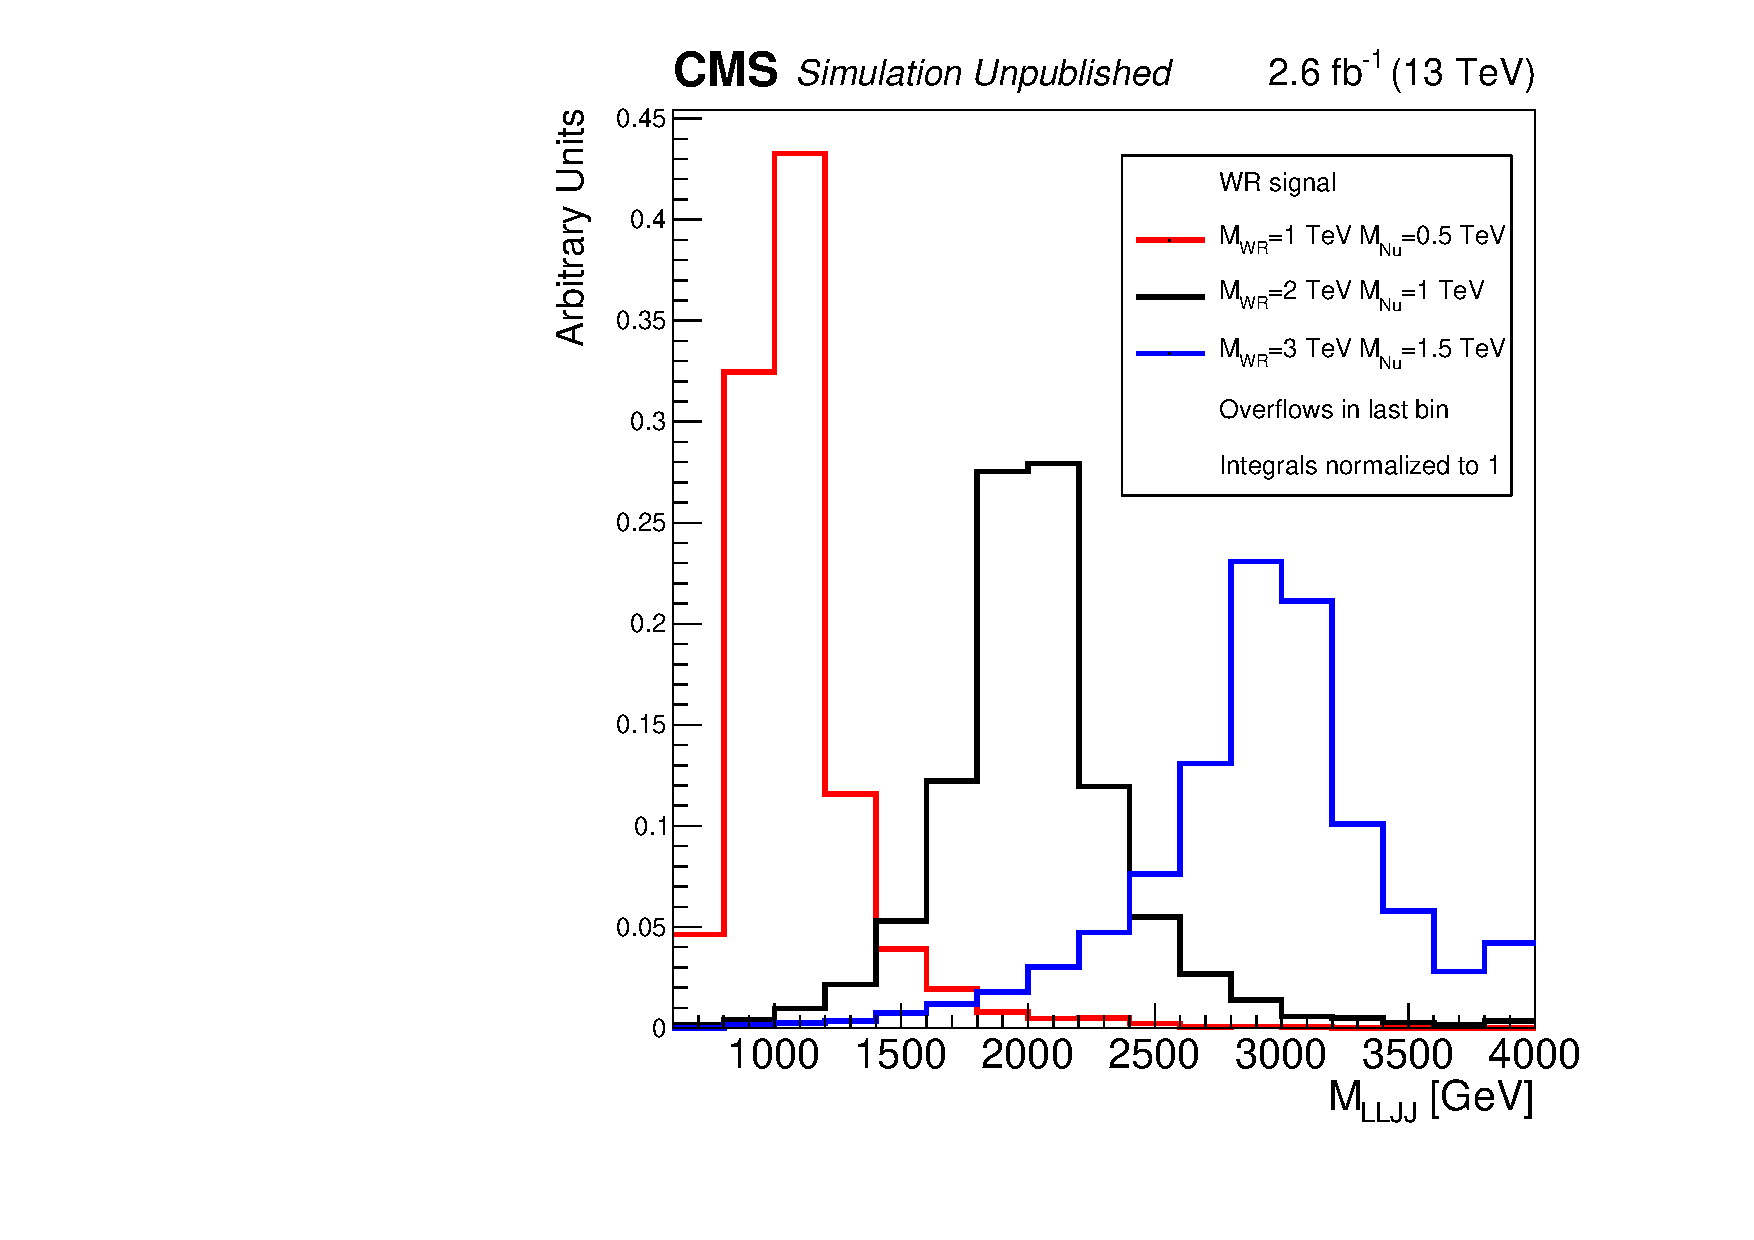
\includegraphics[width=0.65\textwidth]{figures/Mlljj_signalRegionCuts_severalWrSignals_EE.pdf}
	}
	\subfigure{
		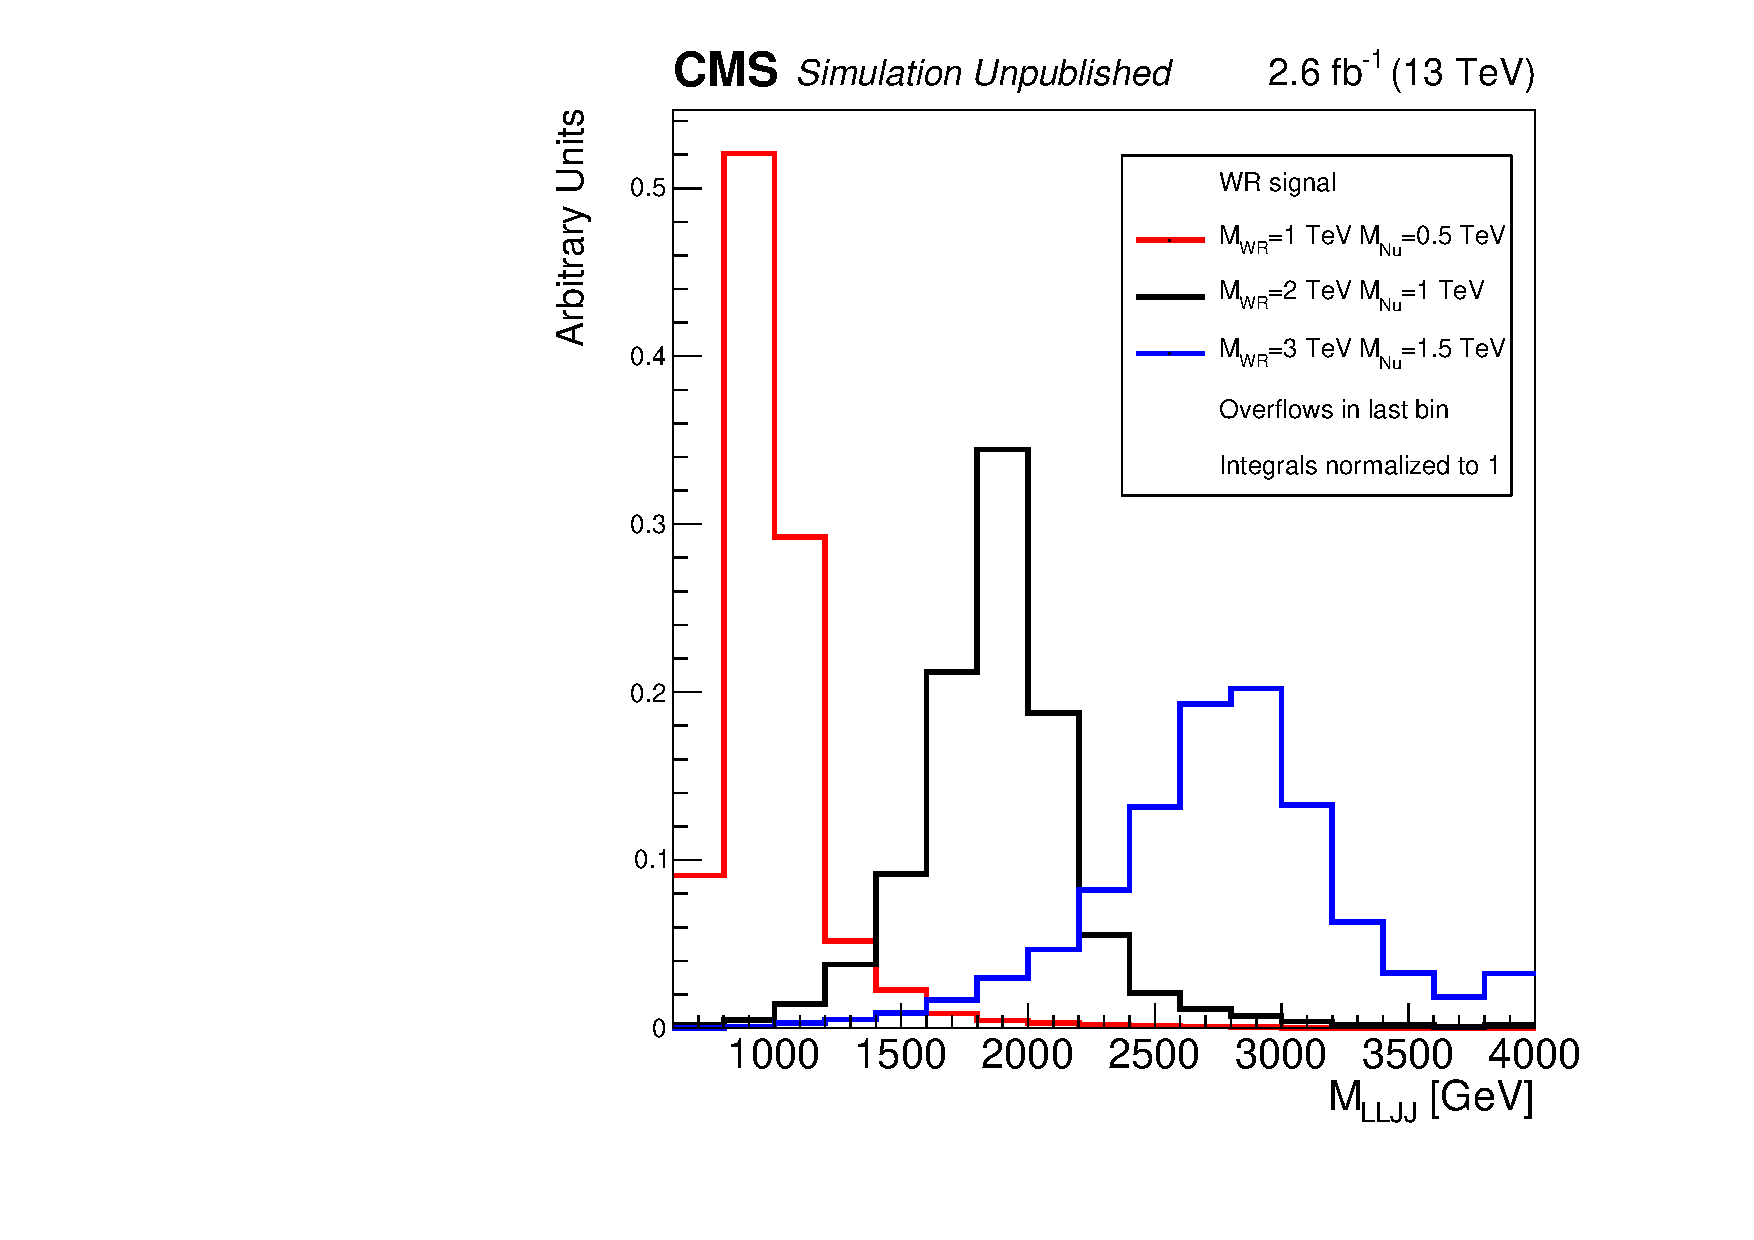
\includegraphics[width=0.65\textwidth]{figures/Mlljj_signalRegionCuts_severalWrSignals_MuMu.pdf}
	}
	\label{fig:signalShapesAfterSelection}
	\caption{The $\Mlljj$ distribution after all selections using simulated \WR signal events with several \mWR hypotheses.  The 
	$ee$- ($\mu\mu$-) channel is shown on the left (right).}
\end{figure}

The optimized windows, listed in Table \ref{tab:masscuts}, overlapped in $\Mlljj$ because 
each selected event could be consistent with several \mWR hypotheses.  In each window the number of selected 
events in data, estimated $\DY$ and top quark backgrounds, and the appropriate \WR simulation\footnote{The window 
optimized for $\mWR = 1000$ $\GeV$ only considered signal events produced in the $\mWR = 1000$ $\GeV$ simulation.} 
were counted, and were used to calculate observed and expected upper limits on $\sigma(\WR) \times BR(\WR \rightarrow \ell\ell jj)$.  
The uncertainties affecting these limits were calculated using procedures described next.

\begin{table}[h]
\caption{$\Mlljj$ window ranges that minimized the expected upper limit on the \WR cross section at different \mWR values.}
\label{tab:masscuts}
\centering
\begin{tabular}{|c|r@{ - }l|r@{ - }l|} \hline
\mWR (\GeV) & \multicolumn{4}{c|}{\Mlljj window (\GeV)}  \\\hline
& \multicolumn{2}{c|}{Electrons}  & \multicolumn{2}{c|}{Muons}  \\  \hline
 800  & 700       &  1100       &  700       &  1200      \\  \hline
1000  & 900       &  1300       &  900       &  1400      \\  \hline
1200  & 1100       &  1550       &  1100       &  1650      \\  \hline
1400  & 1250       &  1750       &  1300       &  1850      \\  \hline
1600  & 1450      &  2000       &  1500      &  2100      \\  \hline
1800  & 1600      &  2250       &  1600      &  2300      \\  \hline
2000  & 1850      &  2550       &  1850      &  2600      \\  \hline
2200  & 2000      &  2800       &  2000      &  2850      \\  \hline
2400  & 2150      &  3100       &  2150      &  3100      \\  \hline
2600  & 2250      &  3400       &  2300      &  3400      \\  \hline
2800  & 2350      &  3700       &  2400      &  3700      \\  \hline
3000  & 2500      &  4000       &  2500      &  3950      \\  \hline
3200  & 2550      &  4300       &  2700      &  4250      \\  \hline
3600  & 2700      &  4900       &  2900      &  4850      \\  \hline
3800  & 2750      &  5200       &  2950      &  5150      \\  \hline
4000  & 2800      &  5500       &  3000      &  5450      \\  \hline
4200  & 2800      &  5750       &  3100      &  5750      \\  \hline
4400  & 2850      &  6050       &  3150      &  6100      \\  \hline
4600  & 2850      &  6300       &  3150      &  6400      \\  \hline
4800  & 2850      &  6600       &  3200      &  6700      \\  \hline
5000  & 2900      &  6850       &  3200      &  7000      \\  \hline
5200  & 2900      &  7050       &  3200      &  7300      \\  \hline
5600  & 2900      &  7500       &  3200      &  7850      \\  \hline
5800  & 2950      &  7700       &  3200      &  8150      \\  \hline
6000  & 2950      &  7900       &  3200      &  8400      \\  \hline
\end{tabular}
\end{table}

%%%%%%%%%%%%%%%%%%%%%%%%%%%%%%%%%%%%%%%%%%%%%%%%%%%%%%%%%%%%%%%%%%%%%%%%%%%%%%%%
% Uncertainties 
%%%%%%%%%%%%%%%%%%%%%%%%%%%%%%%%%%%%%%%%%%%%%%%%%%%%%%%%%%%%%%%%%%%%%%%%%%%%%%%%
\section{Uncertainties}
\label{sec:uncertainties}
%%%%%%%%%%%%%%%%%%%%%%%%%%%%%%%%%%%%%%%%%%%%%%%%%%%%%%%%%%%%%%%%%%%%%%%%%%%%%%%%
The precision of expected and observed limits was reduced by uncertainties on the number of selected signal 
and background events.  In every $\Mlljj$ window the uncertainty magnitudes were estimated and quantified as a 
percentage uncertainty on the number of counted events.

\subsection{Primary Uncertainties}
\label{sec:dominantUncs}

\subsubsection{Energy and Lepton Identification Uncertainties}
\label{sec:enrgyLeptIdUncs}
The only uncertainties that affected the shape of the $\Mlljj$ distribution found in signal and background 
events were uncertainties on the lepton and jet energy resolutions and calibration scales.  The magnitude of 
these uncertainties varied with selected particle kinematic variables like energy and $(\eta,\phi)$ trajectory, 
but never exceeded 25\% for jets, and $\sim$7\% for electrons and muons.  These energy uncertainties changed 
the energies of all reconstructed leptons and jets, and therefore could change the $\Mlljj$ value of a 
selected event, or cause an event to pass (fail) the selection when initially, ignoring energy uncertainties, 
the event failed (passed) the selection.  For convenience, the effect of lepton and jet energy uncertainties 
were estimated simultaneously with the effect of lepton ID uncertainties, which only affected the weight of 
selected simulated events.  Independently considering simulated $\WR$ signal events, simulated $\DY$ events, 
and $e\mu$ data events representing the top quark background, the effect of lepton and jet energy uncertainties 
and lepton ID uncertainties was estimated using the following procedure:

\begin{itemize}
	\item In each event selected by a trigger, but before any lepton or jet selections:
	\begin{itemize}
		\item Eight random numbers were pulled from eight different Gaussians, each with mean 0 and variance 1.
		\item Two random numbers multiplied the electron energy scale and resolution uncertainty of each electron, and these 
			energy changes were propagated to every electron.  In simulated events, a third random number multiplied 
			the ID weight uncertainty of each electron, and the change in weight was propagated to the total event weight 
			after all selections.
		\item Three other random numbers were used to determine the effect of muon energy and ID uncertainties (ID uncertainty 
			only considered in simulated events) following the same procedure used for electrons.
		\item The remaining two random numbers multiplied the jet energy scale and resolution uncertainty of each jet, and 
			these energy changes were propagated to every jet.
	\end{itemize}
	\item The offline selections described in Chapter \ref{sec:event_selection_chapter} were applied to each event.  If all 
		requirements were met and a \WR candidate was built, the event was assigned to one or more $\Mlljj$ windows based on 
		the \WR candidate mass.
\end{itemize}

This procedure was repeated 3200 times for every event.  For each signal and background process, distributions 
of the number of events in each $\Mlljj$ window for all 3200 iterations were made, of which an example  
is shown in Figure \ref{fig:effectOfEnergyIdUncerts}.  The 
distribution's standard deviation represented the uncertainty on the number of events due 
to energy and ID uncertainties.  The uncertainties on the number of signal and background events in one $\Mlljj$ 
window due to energy and ID uncertainties is shown in Table \ref{tab:impactOfEnergyIdUncerts}.  The effect of 
these uncertainties were included in limit calculations by using Gamma distributions for the marginal posterior 
distributions.

\begin{figure}[h]
	\centering
	
\includegraphics[width=1.0\textwidth]{figures/missingImage.png}
	\caption{The number of expected $\WR \rightarrow \mu\mu jj$ signal events with $\mWR = 2.2\TeV$ in the 2.2$\TeV$ 
	$\Mlljj$ window after 3200 iterations of energy and ID uncertainty variations.}
	\label{fig:effectOfEnergyIdUncerts}
\end{figure}

\begin{table}[ht]
	\caption{The effect of energy and ID uncertainties on the number of signal and background events in the $\Mlljj$ 
		window optimized for the $\mWR = 2.2\TeV$ hypothesis.  All uncertainties are in percentages of expected events.  The top 
	quark background estimate is sensitive to $e$ and $\mu$ energy uncertainties.}
  \label{tab:impactOfEnergyIdUncerts}
  \centering
    \begin{tabular}{c|c|c|c}
		Process & Uncertainty sources    & $\Delta(\Neejj)$ (\%) & $\Delta(\Nmumujj)$ (\%)  \\
      \hline
	  \WR & lepton energy and ID & $1$ & $3$ \\ 
	  \WR & jet energy & $1$ & $1$ \\ 
	  \DY &  lepton energy and ID & $4$ & $7$  \\
	  \DY &  jet energy & $14$ & $11$  \\
	 Top quark background & lepton energy & $8$ & $8$ \\
	 Top quark background & jet energy & $2$ & $2$  \\
  \hline
  \end{tabular}
\end{table}

\subsubsection{Statistical Uncertainty}
\label{sec:statUnc}
The statistical uncertainty was calculated for each signal and background source as 
$\sqrt{\sum w_{i}^{2}}$, where $w_{i}$ was the weight of event i, and the sum ran over all selected events 
in a $\Mlljj$ window.  The top quark background was estimated using $e\mu$ data events all with a weight of 
1, while simulated \WR and \DY events had positive weights $<$ 1.  Comparing signal and background statistical 
uncertainties, the statistical uncertainty was largest for the top quark background, as shown in Table 
\ref{tab:impactOfStatUncert}.  No $e\mu$ data events had $\Memujj \geq 2700$ $\GeV$, so the top quark 
background estimate was 0 events for signal hypotheses with $\mWR \geq 3600$ $\GeV$, and the standard 
statistical uncertainty formula could not be used.  In $\Mlljj$ windows where the top quark background estimate 
was 0 events, the statistical uncertainty assigned to 0 events was 1 $e\mu$ event multiplied by the appropriate 
$\ell\ell:e\mu$ normalization factor, 0.659 or 0.432.  The effect of statistical uncertainties were included 
in limit calculations by using Gamma distributions for the marginal posterior distributions.

\begin{table}[ht]
	\caption{Impact of statistical uncertainty on the number of expected signal and background events in the $\Mlljj$ 
		window optimized for the $\mWR = 2.2\TeV$ hypothesis.  All uncertainties are in percentages of expected events.}
  \label{tab:impactOfStatUncert}
  \centering
    \begin{tabular}{c|c|c}
		Process & $\Delta(\Neejj)$ (\%) & $\Delta(\Nmumujj)$ (\%)  \\
      \hline
	  \WR & $1$ & $1$ \\
	  \DY & $6$ & $5$ \\
	 Top quark background & $44$ & $44$  \\
  \hline
  \end{tabular}
\end{table}

\subsubsection{Background Uncertainty from Control Regions}
\label{sec:bkgndNormUnc}
Based on previously discussed comparisons between data and simulated backgrounds in control regions, 
additional uncertainties independent of $\Mlljj$ were applied to background estimates.  A 10\% 
uncertainty was assigned to the top quark background estimate to account for fluctuations in the 
$\ell\ell:e\mu$ normalization factor versus $\Mlljj$.  A 40\% uncertainty was applied to the $\DY$ 
background estimate to account for disagreement between data and simulated $\DY$+jets events in 
the $\Mlljj$ distribution in the low $\Mll$ control region.  The effect of these uncertainties were 
included in limit calculations using log-normal distributions for the marginal posterior distributions.

\subsection{Secondary Uncertainties}
\label{sec:subdominantUncs}

\subsubsection{Lepton Reconstruction and Trigger Efficiency Uncertainties}
\label{sec:leptonRecoTriggerEffUnc}
The efficiencies of lepton reconstruction and muon trigger selections differed between events selected 
in simulations and in data, and these differences were corrected by applying $\sim$unity weights to simulated 
\DY and \WR events.  In the $\mu\mu$-channel, the trigger and lepton reconstruction 
efficiency weights varied with the $\pt$ and $\eta$ of selected muons, and the weight uncertainties 
were statistical uncertainties, determined by the number of data and simulated events used to calculate 
the weights.  The uncertainty on the muon reconstruction efficiency weights was negligible.  The muon 
trigger efficiency weight uncertainty was $<$ 0.5\% for events triggered by muons with $\pt < 140$ $\GeV$.  For 
events triggered by muons with $\pt \geq 140$ $\GeV$, the trigger efficiency weight uncertainty was higher 
because fewer data events were available to calculate the weight: $<$ 3\% uncertainty for triggering 
muons with $|\eta| < 2.1$, and 5.1\% uncertainty for triggering muons with $2.1 < |\eta| < 2.4$.  In 
the $ee$-channel, an electron reconstruction efficiency weight of 0.982 was applied to all selected 
electrons.  The weight uncertainty was 2\%, and was calculated as the maximum difference between 0.982 
and an $\Et,\eta$ dependent weight.  The effect of lepton reconstruction and trigger selection efficiency 
uncertainties were included in limit calculations using log-normal distributions for the marginal posterior 
distributions.

\subsubsection{Cross Section, Luminosity, Pileup and PDF Uncertainties}
\label{sec:crossSxnPileupPdfUnc}
The \DY background and \WR signal were estimated using simulated events whose event weights were 
susceptible to uncertainties on cross sections, pileup, integrated luminosity, parton distribution functions 
(PDFs), and QCD scales.  The \DY cross section uncertainty was 2\% (1\%) in the $ee$- ($\mu\mu$-) channel, 
and was estimated by comparing data to simulated \DY datasets produced with different \MC generators in 
the $Z \rightarrow \ell\ell$ control region discussed earlier.  Treating PDF uncertainties separately, the 
\WR cross section uncertainty was proportional to the uncertainties on the ST top quark mass, and the 
ST $W$ boson coupling strengths to ST fermions.  These ST uncertainties are $<$ 0.5\%, and as a result 
the \WR cross section uncertainty was negligible.

The efficiency in data to reconstruct an interaction as a vertex could not be measured exactly, so an 
analytic, multivariate function was used to approximate this efficiency in data.  This function was used to 
derive the pileup weights\footnote{The pileup weights were equal to the pileup distribution in data 
divided by the pileup distribution in simulated events} $w_{PU}$ applied to simulated events, and uncertainty 
in the function's parameters created uncertainty in $w_{PU}$.  The $w_{PU}$ uncertainty was estimated by 
shifting the pileup distribution in data without changing its shape so that the mean pileup value increased 
or decreased by 5\%.  New pileup weights $w_{PU,\Uparrow}$ and $w_{PU,\Downarrow}$ were calculated after the 
upward and downward shifts, and the $w_{PU}$ uncertainty was calculated as the maximum percentage change in 
events in each $\Mlljj$ window using the original and new weights.  For \DY and \WR event estimates, the pileup 
uncertainty was 3\% or less in all $\Mlljj$ windows.

Knowing the cross sections of the \WR and \DY processes, the numbers of \WR and \DY events were normalized 
to the measured integrated luminosity of data.  The integrated luminosity of data was measured with a 2.7\% 
uncertainty, which translated into a 2.7\% luminosity uncertainty on the number of \WR and \DY events in 
every $\Mlljj$ window.

\DY and \WR events were simulated using:

\begin{itemize}
	\item One parton distribution function (PDF) that described how momenta were distributed amongst quark and 
		gluon constituents of colliding protons.  \WR simulations used NNPDF23 \cite{nnpdf23}, \DY simulations 
		used NNPDF30 \cite{nnpdf30}, and both PDFs were characterized by fixed value coefficients with uncertainties.
	\item One renormalization scale value $\mu_{R}$ (in $\GeV$) that determined the QCD coupling strength $\alpha_{QCD}$.
	\item One factorization scale value $\mu_{F}$ (in $\GeV$), which allowed QCD interactions with low momentum transfer 
		$k_{low} \ll \mu_{F}$ to be simulated independently of QCD interactions with high momentum transfer 
		$k_{high} \sim \mu_{F}$ (explained further in \cite{qcdFactorizationTheory}).
\end{itemize}

The effect of uncertainties in the PDF, $\mu_{R}$ and $\mu_{F}$ values were estimated by resimulating \DY and 
\WR events with different PDF coefficients and QCD scale values, and subsequently reapplying all event selections 
and corrections.  The QCD scales were independently increased or decreased by a factor of 2 
(both were doubled, one was not changed while the other was halved, etc), and the QCD scale uncertainty was the 
maximum percentage change in events in a $\Mlljj$ window.  The PDF coefficients were varied o.

%RESUME HERE

The QCD scale uncertainty was added 
in quadrature with the PDF uncertainty for each $\Mlljj$ window.  For \DY events the combined PDF and QCD 
scale uncertainty never exceeded 4\% in any $\Mlljj$ window.  For each \mWR hypothesis, the PDF and QCD scale 
uncertainty was calculated in the $\Mlljj$ window optimized for the specific \mWR hypothesis.  For all \mWR 
hypotheses the QCD scale uncertainty was no more than a few percent for any \mWR, but the PDF uncertainty 
scaled with \mWR, as shown in Table \ref{tab:wrPdfAndQCDscaleUnc}.  Following CMS guidelines, the \WR PDF 
uncertainty was factored into two pieces: one piece that only depends on relativistic kinematics and masses 
(\mWR and \mnul) and affects the $(\eta, \phi)$ acceptance of \WR decay products, and another piece that depends 
on variable, weakly constrained parameters in LRS models and affects the production rate of \WR bosons.  The acceptance 
uncertainty was $\lesssim$ 1\% for all \mWR hypotheses, and was included in the calculation of results.  The 
production rate uncertainty, constituting the majority of the PDF uncertainty, grew with \mWR, but was not 
included when calculating the results because the uncertainty depended on the LRS model that was chosen.  
In limit calculations the PDF, $\mu_{R}$ and $\mu_{F}$ uncertainties were taken into account using log-normal 
distributions.

The effect of uncertainties on cross sections, pileup, integrated luminosity, PDFs, and QCD scales were included 
in limit calculations using log-normal distributions for the marginal posterior distributions.

\begin{table}[ht]
	\caption{Uncertainty in the number of predicted \WR signal events due to PDF and QCD scale uncertainties.}
  \label{tab:wrPdfAndQCDscaleUnc}
  \centering
    \begin{tabular}{c|c|c}
		\mWR ($\GeV$)             & $\Delta(\Neejj)$ (\%) & $\Delta(\Nmumujj)$ (\%)  \\
      \hline
	  1000  & $4$ & $4$ \\
	  2200 & $7$ & $7$ \\
	  3000 & $15$ & $15$ \\
	  4000 & $18$ & $19$ \\
	  \hline
  \end{tabular}
\end{table}

\subsection{Cumulative Uncertainty}
\label{sec:cumulativeUnc}
The net effect of all uncertainty sources on the estimated number of ST background and \WR signal events in 
several $\Mlljj$ windows is shown in Table \ref{tab:expectedEventsAndAllUncs}.  All uncertainties excluding 
the statistical uncertainty were labeled as systematic uncertainties, and their magnitudes were all summed 
in quadrature.  The dominant \DY background uncertainty was the 40\% uncertainty assigned based on disagreement 
between data and simulated events in a control region where good agreement was expected.  The dominant top 
quark background uncertainty was statistical uncertainty, as fewer than 500 $e\mu$ data events passed the 
full selection with $\Mlljj > 600\GeV$.

\begin{table}[htp]
	\caption{For \mWR hypotheses with $M_{\nul} = \frac{1}{2} \mWR$, these are the number of expected \WR signal and background events in each $\Mlljj$ window, and 
	their statistical and systematic uncertainties.  Each uncertainty is listed as a number of events relative to the expected number of events. BG = Backgrounds, DY = \DY }
	\label{tab:expectedEventsAndAllUncs}
	\centering
	\resizebox{1\textwidth}{3.1cm}{\begin{tabular}{|c|c|c|c|c|}
		& \multicolumn{4}{c|}{Electron channel}  \\
		\mWR ($\GeV$) & Signal (exp $\pm$ stat $\pm$ syst) & DY (exp $\pm$ stat $\pm$ syst) & Top quark (exp $\pm$ stat $\pm$ syst) & $\sum$ BG (exp $\pm$ stat $\pm$ syst) \\\hline
		1000 & 1196.0 $\pm$ 15.0 $\pm$ 46.0 & 21.11 $\pm$ 1.64 $\pm$ 8.79 & 40.87 $\pm$ 4.2 $\pm$ 4.76 & 61.99 $\pm$ 4.51 $\pm$ 10.0   \\ \hline
		2200 & 38.0 $\pm$ 0.4 $\pm$ 1.5 & 2.66 $\pm$ 0.15 $\pm$ 1.16 & 2.25 $\pm$ 0.99 $\pm$ 0.3 & 4.92 $\pm$ 1.0 $\pm$ 1.2    \\ \hline
		3000 & 7.3 $\pm$ 0.07 $\pm$ 0.27 & 1.02 $\pm$ 0.09 $\pm$ 0.44 & 0.43 $\pm$ 0.43 $\pm$ 0.05 & 1.45 $\pm$ 0.44 $\pm$ 0.45    \\ \hline
		4000 & 1.0 $\pm$ 0.01 $\pm$ 0.04 & 0.65 $\pm$ 0.08 $\pm$ 0.29 & 0.0 $\pm$ 0.43 $\pm$ 0.0 & 0.65 $\pm$ 0.44 $\pm$ 0.29    \\ \hline
	   & \multicolumn{4}{c|}{Muon channel}  \\
		\mWR ($\GeV$) & Signal (exp $\pm$ stat $\pm$ syst) & DY (exp $\pm$ stat $\pm$ syst) & Top quark (exp $\pm$ stat $\pm$ syst) & $\sum$ BG (exp $\pm$ stat $\pm$ syst) \\\hline
		1000 & 1805.0 $\pm$ 17.9 $\pm$ 83.1 & 42.16 $\pm$ 2.28 $\pm$ 17.85 & 70.51 $\pm$ 6.82 $\pm$ 7.97 & 112.67 $\pm$ 7.19 $\pm$ 19.55   \\ \hline
		2200 & 52.0 $\pm$ 0.5 $\pm$ 2.5 & 4.97 $\pm$ 0.25 $\pm$ 2.14 & 3.44 $\pm$ 1.51 $\pm$ 0.45 & 8.41 $\pm$ 1.53 $\pm$ 2.18    \\ \hline
		3000 & 9.1 $\pm$ 0.08 $\pm$ 0.39 & 2.62 $\pm$ 0.16 $\pm$ 1.13 & 0.66 $\pm$ 0.66 $\pm$ 0.08 & 3.28 $\pm$ 0.68 $\pm$ 1.13    \\ \hline
		4000 & 1.2 $\pm$ 0.01 $\pm$ 0.05 & 1.37 $\pm$ 0.1 $\pm$ 0.63 & 0.0 $\pm$ 0.66 $\pm$ 0.0 & 1.37 $\pm$ 0.67 $\pm$ 0.63    \\ \hline
	\end{tabular}}
\end{table}


%%%%%%%%%%%%%%%%%%%%%%%%%%%%%%%%%%%%%%%%%%%%%%%%%%%%%%%%%%%%%%%%%%%%%%%%%%%%%%%%
% Results
%%%%%%%%%%%%%%%%%%%%%%%%%%%%%%%%%%%%%%%%%%%%%%%%%%%%%%%%%%%%%%%%%%%%%%%%%%%%%%%%
\section{Results}
\label{sec:searchResults}
Evidence of LRS models was searched for by comparing expected signal and background events to observed data 
events after all selections.  Initial results were obtained by inspecting the $\Meejj$ and $\Mmumujj$ 
distributions with (Table \ref{tab:expAndObsEvtsWithAllUncs}) and without (Figure \ref{fig:obsAndExpMlljj}) 
the $\Mlljj$ window cuts.  No statistically significant excess was observed in data with respect to expected 
backgrounds, so limits were calculated on $\sigma(\WR) \times BR(\WR \rightarrow \ell\ell jj)$, and \mWR and \mnul.

\begin{table}[htp]
	\caption{For \mWR hypotheses with $M_{\nul} = \frac{1}{2} \mWR$, these are the number of expected \WR signal and background events in each $\Mlljj$ window, and 
	their statistical and systematic uncertainties.  Each uncertainty is listed as a number of events relative to the expected number of events. BG = Backgrounds, DY = \DY }
	\label{tab:expAndObsEvtsWithAllUncs}
	\centering
	\resizebox{1\textwidth}{9cm}{\begin{tabular}{|c|c|c|c|c|c|}
			& \multicolumn{5}{c|}{Electron channel}  \\
			\mWR ($\GeV$) & Signal (exp $\pm$ stat $\pm$ syst) & DY (exp $\pm$ stat $\pm$ syst) & Top quark (exp $\pm$ stat $\pm$ syst) & $\sum$ BG (exp $\pm$ stat $\pm$ syst) & Data \\\hline
			800 & 2690.0 $\pm$ 36.4 $\pm$ 103.4 & 37.95 $\pm$ 2.54 $\pm$ 15.69 & 107.52 $\pm$ 6.81 $\pm$ 11.62 & 145.48 $\pm$ 7.27 $\pm$ 19.52 & 136.0   \\ \hline
			1000 & 1196.0 $\pm$ 15.0 $\pm$ 46.0 & 21.11 $\pm$ 1.64 $\pm$ 8.79 & 40.87 $\pm$ 4.2 $\pm$ 4.76 & 61.99 $\pm$ 4.51 $\pm$ 10.0 & 64.0    \\ \hline
			1200 & 583.0 $\pm$ 7.2 $\pm$ 23.0 & 14.31 $\pm$ 1.3 $\pm$ 5.9 & 24.25 $\pm$ 3.23 $\pm$ 2.58 & 38.56 $\pm$ 3.49 $\pm$ 6.43 & 43.0    \\ \hline
			1400 & 327.0 $\pm$ 3.8 $\pm$ 12.3 & 10.67 $\pm$ 0.99 $\pm$ 4.44 & 16.15 $\pm$ 2.64 $\pm$ 1.79 & 26.82 $\pm$ 2.82 $\pm$ 4.79 & 23.0    \\ \hline
			1600 & 179.0 $\pm$ 2.0 $\pm$ 6.9 & 7.48 $\pm$ 0.7 $\pm$ 3.12 & 5.96 $\pm$ 1.6 $\pm$ 0.75 & 13.44 $\pm$ 1.75 $\pm$ 3.21 & 10.0    \\ \hline
			1800 & 108.0 $\pm$ 1.2 $\pm$ 4.1 & 5.8 $\pm$ 0.6 $\pm$ 2.52 & 3.05 $\pm$ 1.15 $\pm$ 0.42 & 8.85 $\pm$ 1.29 $\pm$ 2.56 & 6.0     \\ \hline
			2000 & 59.0 $\pm$ 0.6 $\pm$ 2.4 & 3.56 $\pm$ 0.2 $\pm$ 1.49 & 2.21 $\pm$ 0.98 $\pm$ 0.32 & 5.77 $\pm$ 1.0 $\pm$ 1.52 & 1.0     \\ \hline
			2200 & 38.0 $\pm$ 0.4 $\pm$ 1.5 & 2.66 $\pm$ 0.15 $\pm$ 1.16 & 2.25 $\pm$ 0.99 $\pm$ 0.3 & 4.92 $\pm$ 1.0 $\pm$ 1.2 & 2.0     \\ \hline
			2400 & 24.6 $\pm$ 0.26 $\pm$ 0.97 & 1.9 $\pm$ 0.13 $\pm$ 0.87 & 2.1 $\pm$ 0.95 $\pm$ 0.26 & 4.0 $\pm$ 0.96 $\pm$ 0.91 & 3.0     \\ \hline
			2600 & 16.3 $\pm$ 0.17 $\pm$ 0.61 & 1.58 $\pm$ 0.14 $\pm$ 0.7 & 1.43 $\pm$ 0.78 $\pm$ 0.29 & 3.01 $\pm$ 0.79 $\pm$ 0.76 & 2.0     \\ \hline
			2800 & 11.2 $\pm$ 0.11 $\pm$ 0.42 & 1.35 $\pm$ 0.13 $\pm$ 0.59 & 0.47 $\pm$ 0.45 $\pm$ 0.13 & 1.82 $\pm$ 0.46 $\pm$ 0.6 & 2.0     \\ \hline
			3000 & 7.3 $\pm$ 0.07 $\pm$ 0.27 & 1.02 $\pm$ 0.09 $\pm$ 0.44 & 0.43 $\pm$ 0.43 $\pm$ 0.05 & 1.45 $\pm$ 0.44 $\pm$ 0.45 & 2.0     \\ \hline
			3200 & 4.8 $\pm$ 0.05 $\pm$ 0.18 & 0.96 $\pm$ 0.09 $\pm$ 0.42 & 0.34 $\pm$ 0.34 $\pm$ 0.18 & 1.3 $\pm$ 0.35 $\pm$ 0.46 & 2.0     \\ \hline
			3600 & 2.1 $\pm$ 0.02 $\pm$ 0.08 & 0.76 $\pm$ 0.09 $\pm$ 0.35 & 0.0 $\pm$ 0.43 $\pm$ 0.0 & 0.76 $\pm$ 0.44 $\pm$ 0.35 & 1.0     \\ \hline
			3800 & 1.5 $\pm$ 0.01 $\pm$ 0.05 & 0.71 $\pm$ 0.09 $\pm$ 0.32 & 0.0 $\pm$ 0.43 $\pm$ 0.0 & 0.71 $\pm$ 0.44 $\pm$ 0.32 & 1.0     \\ \hline
			4000 & 1.0 $\pm$ 0.01 $\pm$ 0.04 & 0.65 $\pm$ 0.08 $\pm$ 0.29 & 0.0 $\pm$ 0.43 $\pm$ 0.0 & 0.65 $\pm$ 0.44 $\pm$ 0.29 & 1.0     \\ \hline
			4200 & 0.7 $\pm$ 0.01 $\pm$ 0.02 & 0.66 $\pm$ 0.08 $\pm$ 0.3 & 0.0 $\pm$ 0.43 $\pm$ 0.0 & 0.66 $\pm$ 0.44 $\pm$ 0.3 & 1.0     \\ \hline
			4400 & 0.44 $\pm$ 0.0042 $\pm$ 0.0163 & 0.61 $\pm$ 0.08 $\pm$ 0.27 & 0.0 $\pm$ 0.43 $\pm$ 0.0 & 0.61 $\pm$ 0.44 $\pm$ 0.27 & 1.0     \\ \hline
			4600 & 0.29 $\pm$ 0.0028 $\pm$ 0.0109 & 0.61 $\pm$ 0.08 $\pm$ 0.28 & 0.0 $\pm$ 0.43 $\pm$ 0.0 & 0.61 $\pm$ 0.44 $\pm$ 0.28 & 1.0     \\ \hline
			4800 & 0.2 $\pm$ 0.0019 $\pm$ 0.0074 & 0.61 $\pm$ 0.08 $\pm$ 0.28 & 0.0 $\pm$ 0.43 $\pm$ 0.0 & 0.61 $\pm$ 0.44 $\pm$ 0.28 & 1.0     \\ \hline
			5000 & 0.14 $\pm$ 0.0013 $\pm$ 0.005 & 0.56 $\pm$ 0.08 $\pm$ 0.26 & 0.0 $\pm$ 0.43 $\pm$ 0.0 & 0.56 $\pm$ 0.44 $\pm$ 0.26 & 1.0     \\ \hline
			5200 & 0.09 $\pm$ 0.0008 $\pm$ 0.0033 & 0.56 $\pm$ 0.08 $\pm$ 0.26 & 0.0 $\pm$ 0.43 $\pm$ 0.0 & 0.56 $\pm$ 0.44 $\pm$ 0.26 & 1.0     \\ \hline
			5600 & 0.04 $\pm$ 0.0004 $\pm$ 0.0015 & 0.56 $\pm$ 0.08 $\pm$ 0.26 & 0.0 $\pm$ 0.43 $\pm$ 0.0 & 0.56 $\pm$ 0.44 $\pm$ 0.26 & 1.0     \\ \hline
			5800 & 0.03 $\pm$ 0.0002 $\pm$ 0.001 & 0.51 $\pm$ 0.08 $\pm$ 0.23 & 0.0 $\pm$ 0.43 $\pm$ 0.0 & 0.51 $\pm$ 0.44 $\pm$ 0.23 & 1.0     \\ \hline
			6000 & 0.02 $\pm$ 0.0002 $\pm$ 0.0007 & 0.51 $\pm$ 0.08 $\pm$ 0.23 & 0.0 $\pm$ 0.43 $\pm$ 0.0 & 0.51 $\pm$ 0.44 $\pm$ 0.23 & 1.0     \\ \hline
		& \multicolumn{5}{c|}{Muon channel}  \\
			\mWR ($\GeV$) & Signal (exp $\pm$ stat $\pm$ syst) & DY (exp $\pm$ stat $\pm$ syst) & Top quark (exp $\pm$ stat $\pm$ syst) & $\sum$ BG (exp $\pm$ stat $\pm$ syst) & Data \\\hline
			800 & 3966.0 $\pm$ 44.4 $\pm$ 176.2 & 73.29 $\pm$ 6.11 $\pm$ 30.45 & 174.32 $\pm$ 10.72 $\pm$ 18.79 & 247.61 $\pm$ 12.34 $\pm$ 35.78 & 244.0   \\ \hline
			1000 & 1805.0 $\pm$ 17.9 $\pm$ 83.1 & 42.16 $\pm$ 2.28 $\pm$ 17.85 & 70.51 $\pm$ 6.82 $\pm$ 7.97 & 112.67 $\pm$ 7.19 $\pm$ 19.55 & 121.0   \\ \hline
			1200 & 872.0 $\pm$ 8.1 $\pm$ 43.4 & 24.23 $\pm$ 1.74 $\pm$ 10.07 & 38.5 $\pm$ 5.04 $\pm$ 4.07 & 62.73 $\pm$ 5.33 $\pm$ 10.86 & 57.0    \\ \hline
			1400 & 441.0 $\pm$ 4.0 $\pm$ 22.9 & 17.04 $\pm$ 1.42 $\pm$ 7.02 & 18.94 $\pm$ 3.53 $\pm$ 2.06 & 35.98 $\pm$ 3.81 $\pm$ 7.32 & 24.0    \\ \hline
			1600 & 244.0 $\pm$ 2.2 $\pm$ 13.3 & 12.71 $\pm$ 1.01 $\pm$ 5.31 & 6.56 $\pm$ 2.07 $\pm$ 1.08 & 19.27 $\pm$ 2.31 $\pm$ 5.42 & 17.0    \\ \hline
			1800 & 150.0 $\pm$ 1.3 $\pm$ 6.7 & 10.94 $\pm$ 0.41 $\pm$ 4.66 & 5.24 $\pm$ 1.86 $\pm$ 0.68 & 16.18 $\pm$ 1.9 $\pm$ 4.71 & 12.0    \\ \hline
			2000 & 82.0 $\pm$ 0.7 $\pm$ 4.3 & 6.52 $\pm$ 0.29 $\pm$ 2.81 & 3.44 $\pm$ 1.51 $\pm$ 0.45 & 9.96 $\pm$ 1.53 $\pm$ 2.85 & 8.0     \\ \hline
			2200 & 52.0 $\pm$ 0.5 $\pm$ 2.5 & 4.97 $\pm$ 0.25 $\pm$ 2.14 & 3.44 $\pm$ 1.51 $\pm$ 0.45 & 8.41 $\pm$ 1.53 $\pm$ 2.18 & 5.0     \\ \hline
			2400 & 32.5 $\pm$ 0.28 $\pm$ 1.52 & 3.89 $\pm$ 0.21 $\pm$ 1.69 & 3.2 $\pm$ 1.45 $\pm$ 0.4 & 7.1 $\pm$ 1.47 $\pm$ 1.74 & 4.0     \\ \hline
			2600 & 20.9 $\pm$ 0.18 $\pm$ 0.97 & 3.28 $\pm$ 0.17 $\pm$ 1.4 & 1.31 $\pm$ 0.92 $\pm$ 0.27 & 4.59 $\pm$ 0.94 $\pm$ 1.42 & 4.0     \\ \hline
			2800 & 13.8 $\pm$ 0.12 $\pm$ 0.6 & 2.97 $\pm$ 0.17 $\pm$ 1.28 & 0.66 $\pm$ 0.66 $\pm$ 0.18 & 3.63 $\pm$ 0.68 $\pm$ 1.29 & 4.0     \\ \hline
			3000 & 9.1 $\pm$ 0.08 $\pm$ 0.39 & 2.62 $\pm$ 0.16 $\pm$ 1.13 & 0.66 $\pm$ 0.66 $\pm$ 0.08 & 3.28 $\pm$ 0.68 $\pm$ 1.13 & 4.0     \\ \hline
			3200 & 5.9 $\pm$ 0.05 $\pm$ 0.26 & 1.99 $\pm$ 0.13 $\pm$ 0.9 & 0.0 $\pm$ 0.66 $\pm$ 0.0 & 1.99 $\pm$ 0.67 $\pm$ 0.9 & 1.0     \\ \hline
			3600 & 2.6 $\pm$ 0.02 $\pm$ 0.11 & 1.52 $\pm$ 0.12 $\pm$ 0.69 & 0.0 $\pm$ 0.66 $\pm$ 0.0 & 1.52 $\pm$ 0.67 $\pm$ 0.69 & 1.0     \\ \hline
			3800 & 1.8 $\pm$ 0.02 $\pm$ 0.07 & 1.46 $\pm$ 0.12 $\pm$ 0.66 & 0.0 $\pm$ 0.66 $\pm$ 0.0 & 1.46 $\pm$ 0.67 $\pm$ 0.66 & 1.0     \\ \hline
			4000 & 1.2 $\pm$ 0.01 $\pm$ 0.05 & 1.37 $\pm$ 0.1 $\pm$ 0.63 & 0.0 $\pm$ 0.66 $\pm$ 0.0 & 1.37 $\pm$ 0.67 $\pm$ 0.63 & 1.0     \\ \hline
			4200 & 0.8 $\pm$ 0.01 $\pm$ 0.03 & 1.21 $\pm$ 0.1 $\pm$ 0.55 & 0.0 $\pm$ 0.66 $\pm$ 0.0 & 1.21 $\pm$ 0.67 $\pm$ 0.55 & 1.0     \\ \hline
			4400 & 0.54 $\pm$ 0.0045 $\pm$ 0.0223 & 1.13 $\pm$ 0.09 $\pm$ 0.52 & 0.0 $\pm$ 0.66 $\pm$ 0.0 & 1.13 $\pm$ 0.67 $\pm$ 0.52 & 1.0     \\ \hline
			4600 & 0.37 $\pm$ 0.003 $\pm$ 0.0151 & 1.14 $\pm$ 0.09 $\pm$ 0.53 & 0.0 $\pm$ 0.66 $\pm$ 0.0 & 1.14 $\pm$ 0.67 $\pm$ 0.53 & 1.0     \\ \hline
			4800 & 0.24 $\pm$ 0.002 $\pm$ 0.0101 & 1.06 $\pm$ 0.08 $\pm$ 0.5 & 0.0 $\pm$ 0.66 $\pm$ 0.0 & 1.06 $\pm$ 0.66 $\pm$ 0.5 & 1.0     \\ \hline
			5000 & 0.18 $\pm$ 0.0014 $\pm$ 0.0074 & 1.06 $\pm$ 0.08 $\pm$ 0.5 & 0.0 $\pm$ 0.66 $\pm$ 0.0 & 1.06 $\pm$ 0.66 $\pm$ 0.5 & 1.0     \\ \hline
			5200 & 0.12 $\pm$ 0.0009 $\pm$ 0.0048 & 1.06 $\pm$ 0.08 $\pm$ 0.5 & 0.0 $\pm$ 0.66 $\pm$ 0.0 & 1.06 $\pm$ 0.66 $\pm$ 0.5 & 1.0     \\ \hline
			5600 & 0.05 $\pm$ 0.0004 $\pm$ 0.0022 & 1.06 $\pm$ 0.08 $\pm$ 0.5 & 0.0 $\pm$ 0.66 $\pm$ 0.0 & 1.06 $\pm$ 0.66 $\pm$ 0.5 & 1.0     \\ \hline
			5800 & 0.04 $\pm$ 0.0003 $\pm$ 0.0015 & 1.06 $\pm$ 0.08 $\pm$ 0.5 & 0.0 $\pm$ 0.66 $\pm$ 0.0 & 1.06 $\pm$ 0.66 $\pm$ 0.5 & 1.0     \\ \hline
			6000 & 0.02 $\pm$ 0.0002 $\pm$ 0.001 & 1.06 $\pm$ 0.08 $\pm$ 0.5 & 0.0 $\pm$ 0.66 $\pm$ 0.0 & 1.06 $\pm$ 0.66 $\pm$ 0.5 & 1.0     \\ \hline
	\end{tabular}}
\end{table}

\begin{figure}[btp]
	\centering
	\subfigure{
		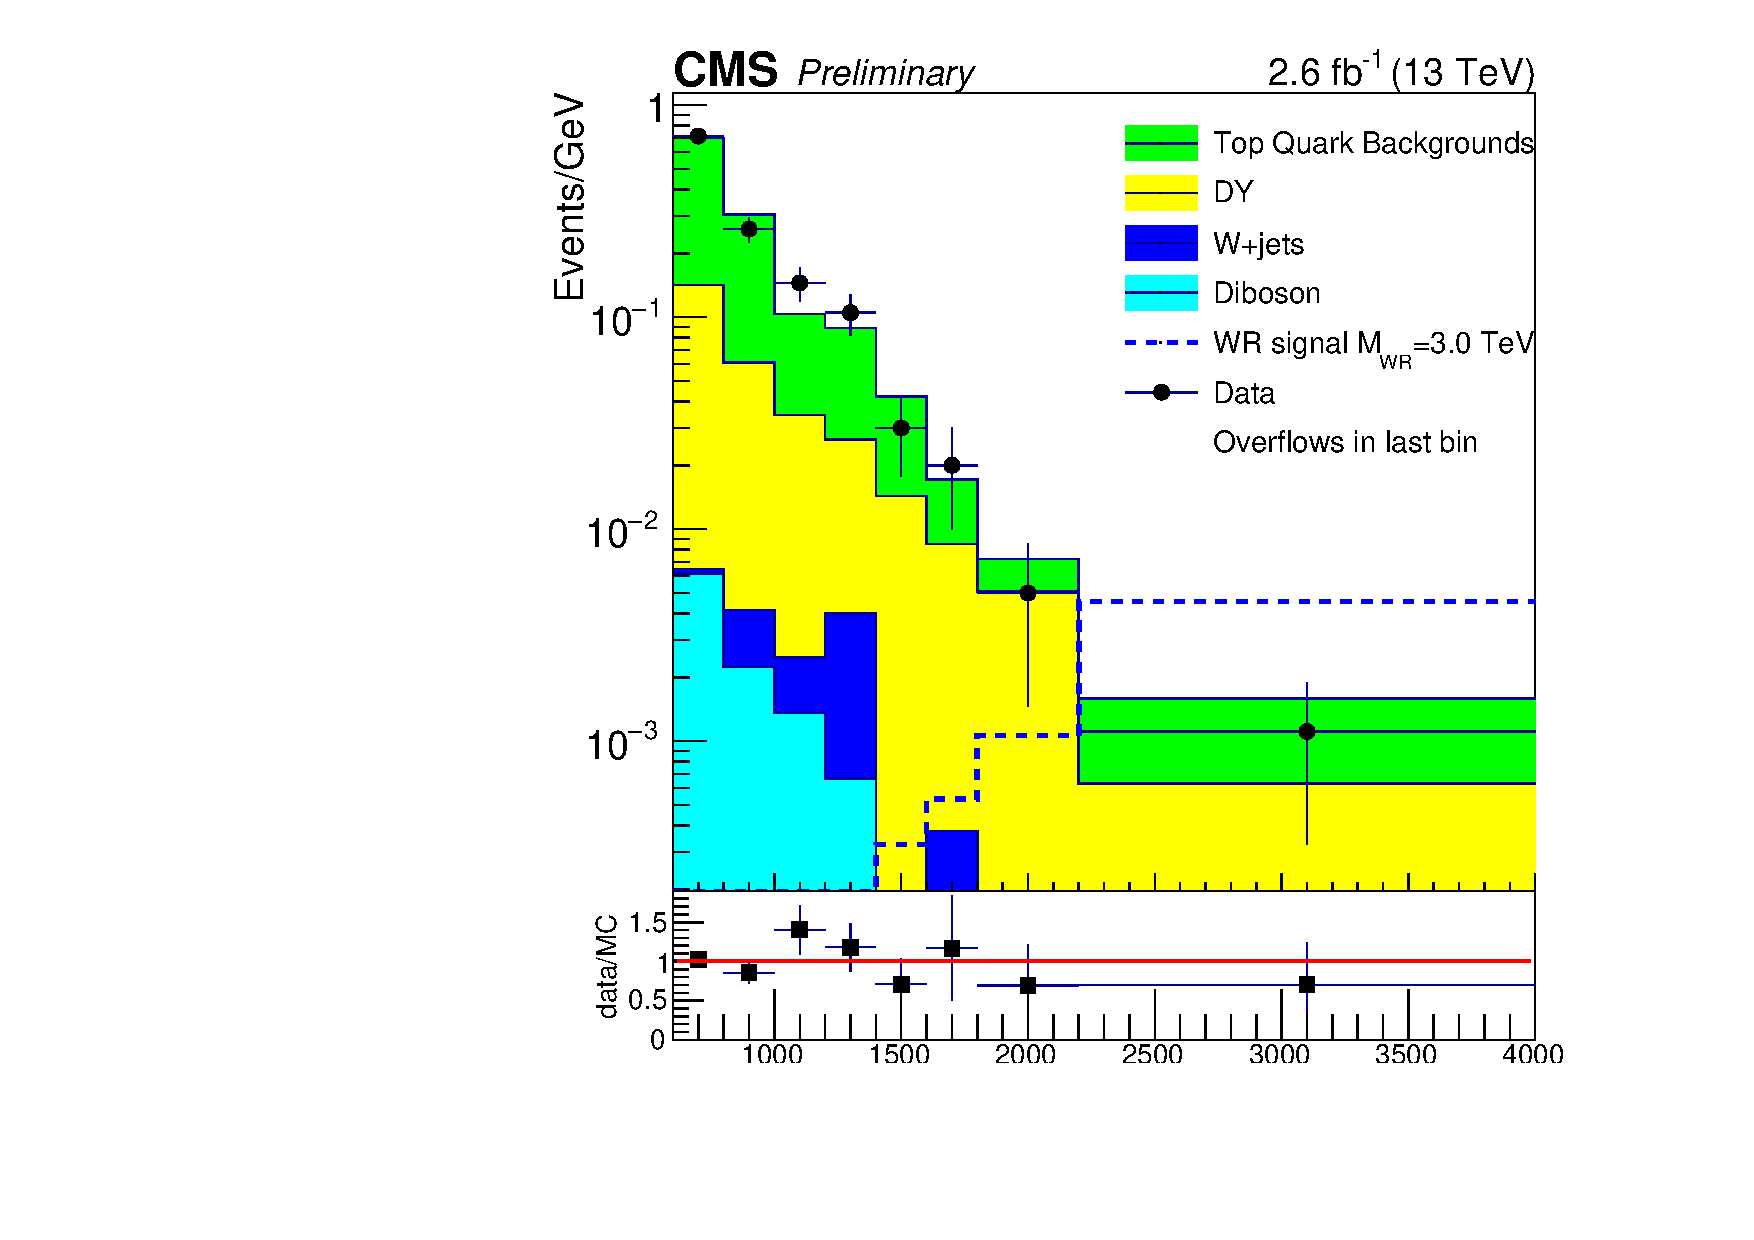
\includegraphics[width=0.65\textwidth]{figures/Mlljj_2012Bins_MWR3000Signal_SignalRegion_EEChannelBkgndMC_DYMadHTAndIncl_TTBarFromData_WithUnblindedData_withRatio_log.pdf}
	}
	\subfigure{
		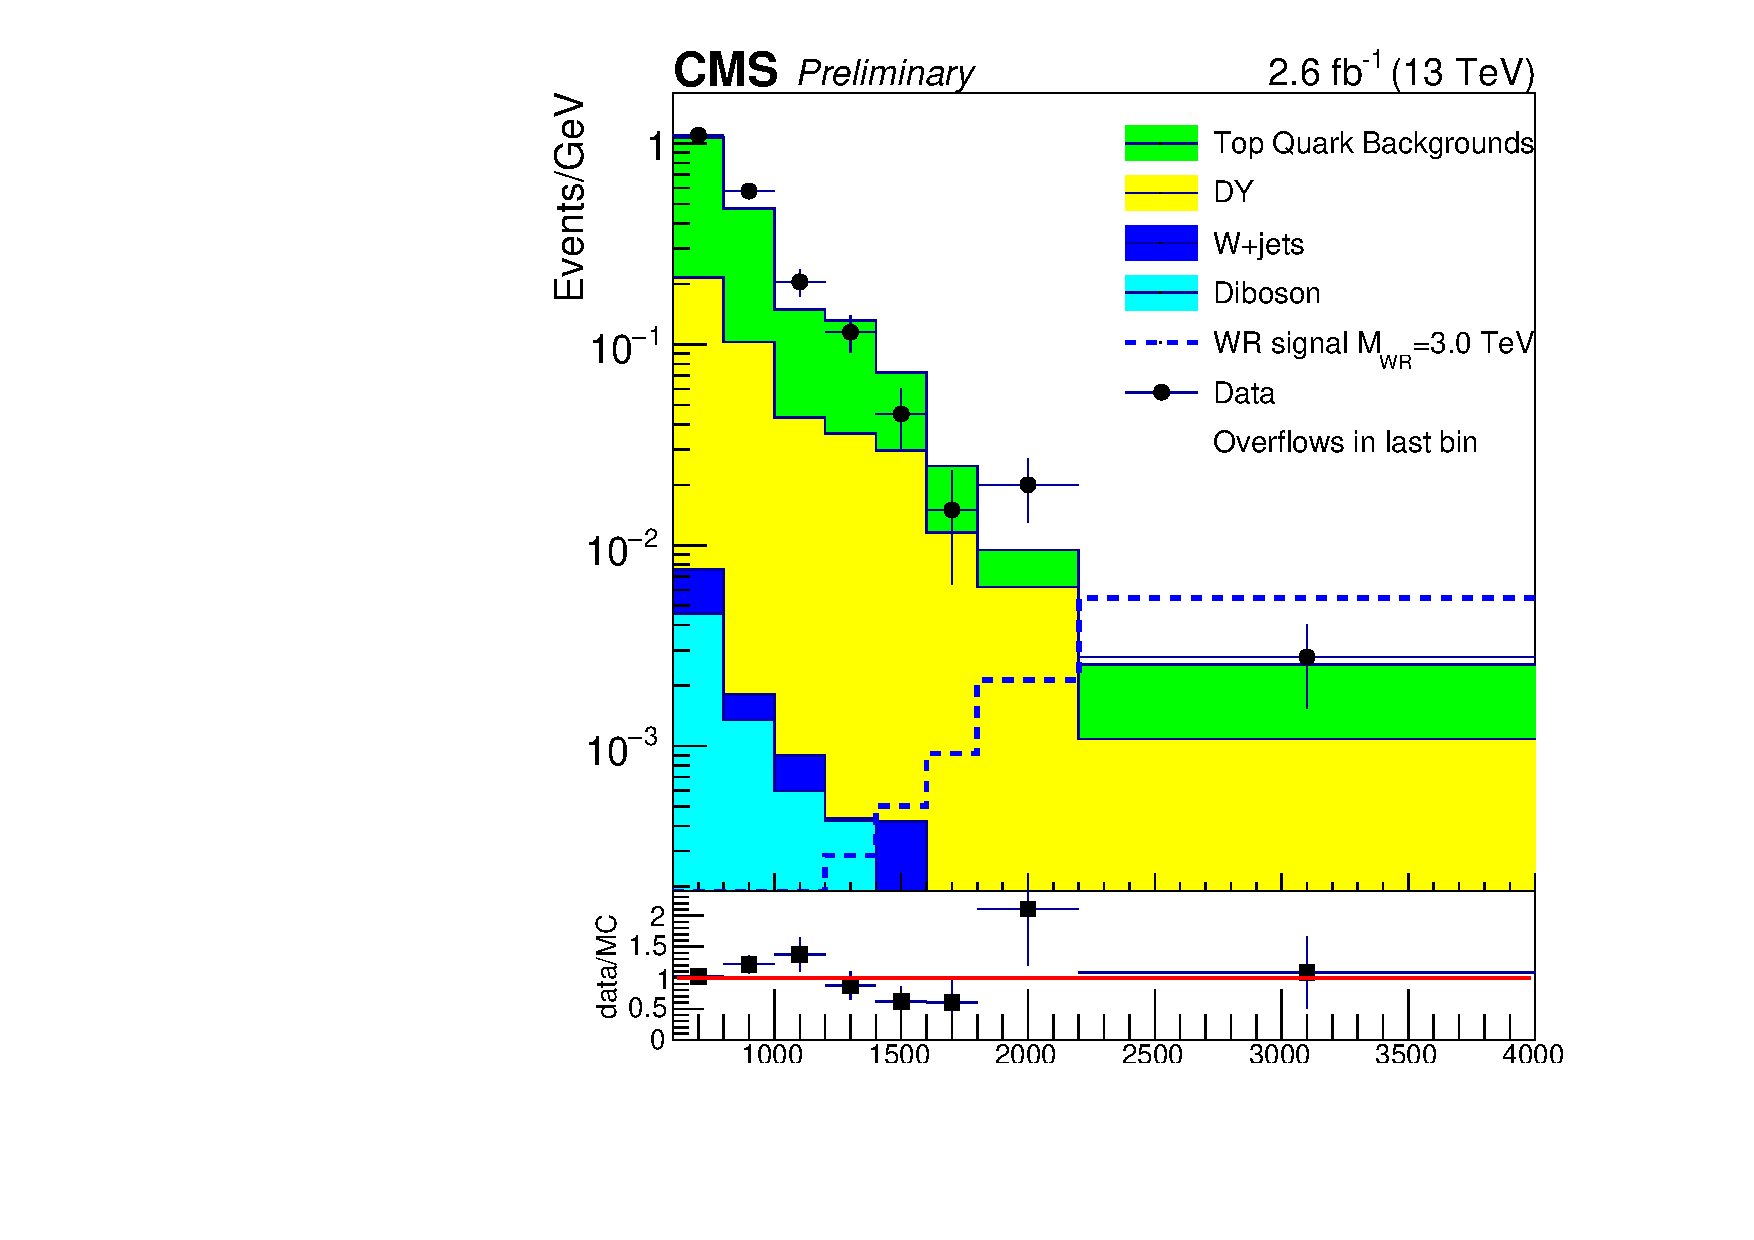
\includegraphics[width=0.65\textwidth]{figures/Mlljj_2012Bins_MWR3000Signal_SignalRegion_MuMuChannelBkgndMC_DYMadHTAndIncl_TTBarFromData_WithUnblindedData_withRatio_log.pdf}
	}
	\label{fig:obsAndExpMlljj}
	\caption{$\Mlljj$ distributions found in data, \WR simulations, and expected backgrounds.  The $ee$ ($\mu\mu$) channel is shown on 
		the left (right).}
\end{figure}

Upper limits on $\sigma(\WR) \times BR(\WR \rightarrow \ell\ell jj)$ at 95\% CL were calculated in each $\Mlljj$ 
window with all uncertainties taken into account, and assuming $\mnul = \frac{1}{2}\mWR$.  Expected limits were 
calculated by setting the measured number of events $\Nlljj$ equal to the expected number of background events, 
and observed limits were calculated by setting $\Nlljj$ equal to the number of events observed in data.  The 
expected and observed limit as a function of \mWR is shown in Figure \ref{fig:oneDimLimits}.  Subsequently, limits 
on $\sigma(\WR) \times BR(\WR \rightarrow \ell\ell jj)$ for fixed $\mnul = \frac{1}{2}\mWR$ were extrapolated into 
\mnul and \mWR exclusion limits using a procedure described next.

\begin{figure}[btp]
	\centering
	\subfigure{
		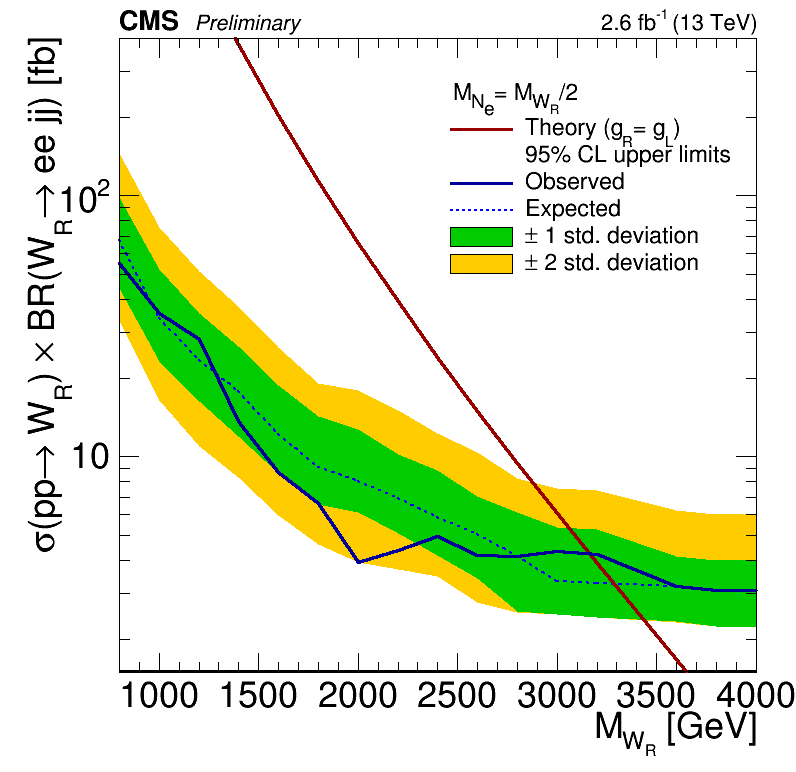
\includegraphics[width=0.65\textwidth]{figures/limWReejj_SHv19700toysAprilTwentyThree.png}
	}
	\subfigure{
		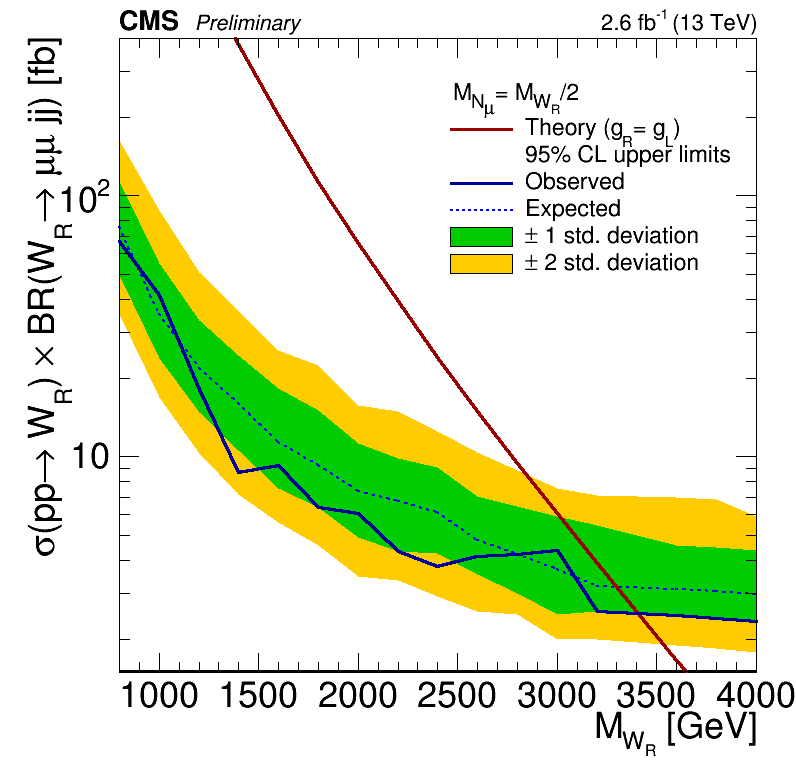
\includegraphics[width=0.65\textwidth]{figures/limWRmumujj_SHv19700toysAprilTwentyThree.png}
	}
	\label{fig:oneDimLimits}
	\caption{Limits on $\sigma(\WR) \times BR(\WR \rightarrow \ell\ell jj)$ at 95\% CL versus \mWR hypothesis.  The $ee$ ($\mu\mu$) channel 
	is shown on the left (right).}
\end{figure}

The limits on $\sigma(\WR) \times BR(\WR \rightarrow \ell\ell jj)$ for fixed $\mnul = \frac{1}{2}\mWR$ are proportional 
to the \WR signal efficiency $\chi$ of the event selection, but are not dependent on the shape of the \WR signal distribution 
within any $\Mlljj$ window.  Thus, a limit at $(\mWR^{a}, \mnul^{a} = \frac{1}{2}\mWR^{a})$ can be extrapolated to a limit at any 
other point $(\mWR^{b}, \mnul^{b} \neq \frac{1}{2}\mWR^{b})$ by knowing the difference in signal efficiency $\chi$ between the two 
points:

%no type of multiplication sign looks good between the fraction and the Limit written on the right side of this equation
\begin{equation}
	Limit[(\mWR^{b}, \mnul^{b} \neq \frac{1}{2}\mWR^{b})] = \frac{\chi[(\mWR^{b}, \mnul^{b} \neq \frac{1}{2}\mWR^{b})]}{\chi[(\mWR^{a}, \mnul^{a} = \frac{1}{2}\mWR^{a})]} \quad Limit[(\mWR^{a}, \mnul^{a} = \frac{1}{2}\mWR^{a})]
\label{eq:limitExtrapolation}
\end{equation}

The dependence of $\chi$ on \mnul and \mWR was estimated first by simulating additional $\WR \rightarrow \ell\ell jj$ 
samples with \mWR between 800 and 4000 $\GeV$, and many values of \mnul between 0 $\GeV$ and \mWR at each value of \mWR.  
%in steps of:
%\begin{itemize}
%	\item 25 $\GeV$ from 0 to 300 $\GeV$,
%	\item 100 $\GeV$ from 300 to $\mWR - 200$ $\GeV$,
%	\item 25 $\GeV$ from $\mWR - 200$ to \mWR $\GeV$
%\end{itemize}
%Smaller steps were used in regions where $\chi$ had a strong dependence on \mnul.
The traditional full simulation used to make \WR samples with $\mnul = \frac{1}{2}\mWR$ required enormous computational resources 
that were not available for the limit extrapolation procedure described here.  Instead, additional \WR 
simulations needed to estimate $\chi$ were produced using only the first simulation step.  \PYTHIA simulated the 
\WR production and decay into leptons and quarks, and the hadronization of quarks into jets.  Similar to reconstructed jets, 
jets from \PYTHIA were clustered from individual hadrons, leptons and photons in a cone of radius $\Delta R =$ 0.4.  After 
event generation and jet clustering, the same selection used in fully reconstructed events was applied, excluding trigger, lepton and jet ID 
selections.  The efficiency of this selection $\chi^'$ was measured as a function of $(\mWR, \mnul)$, and used in place of $\chi$.  
Then the limits on $\sigma(\WR) \times BR(\WR \rightarrow \ell\ell jj)$ calculated for $(\mWR, \mnul = \frac{1}{2}\mWR)$ 
were extrapolated to limits $L'$ for $(\mWR, \mnul \neq \frac{1}{2}\mWR)$ using $\chi^'$ and Equation \ref{eq:limitExtrapolation}.  
The resulting $\sigma(\WR) \times BR(\WR \rightarrow \ell\ell jj)$ limits were reintepreted as 95\% CL exclusion limits on 
the maximum and minimum \mnul masses for each \mWR, and these mass exclusion limits are shown in Figure \ref{fig:twoDimLimits}.

\begin{figure}[tp]
  \centering
  
  \subfigure{
    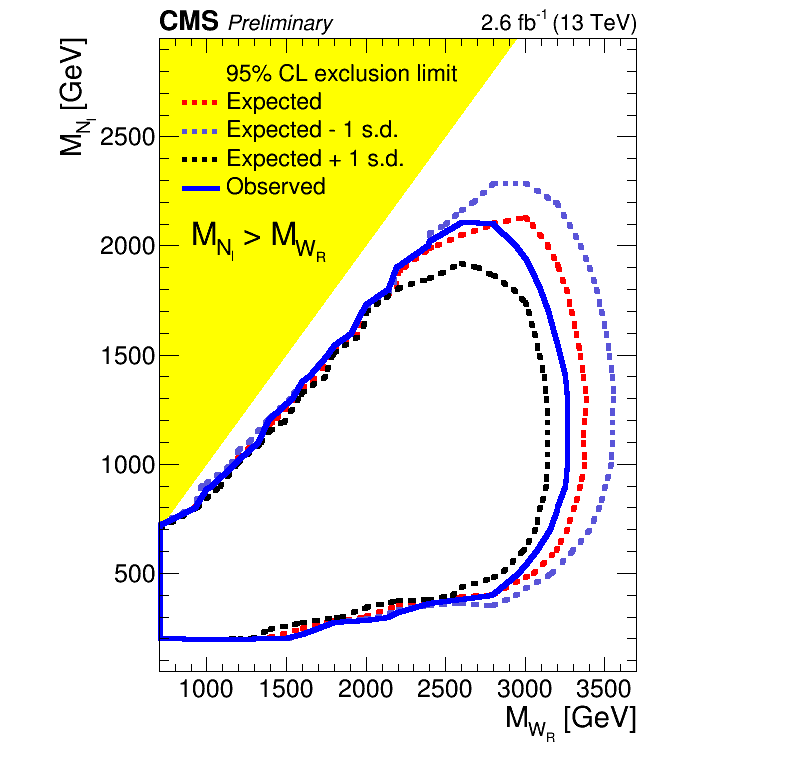
\includegraphics[width=0.65\textwidth]{figures/lim2dWReejj_SHv19700toysAprilTwentyThree_exclusionOverlayWithExpPlusMinusOneSigma.png}
  }
  \subfigure{
    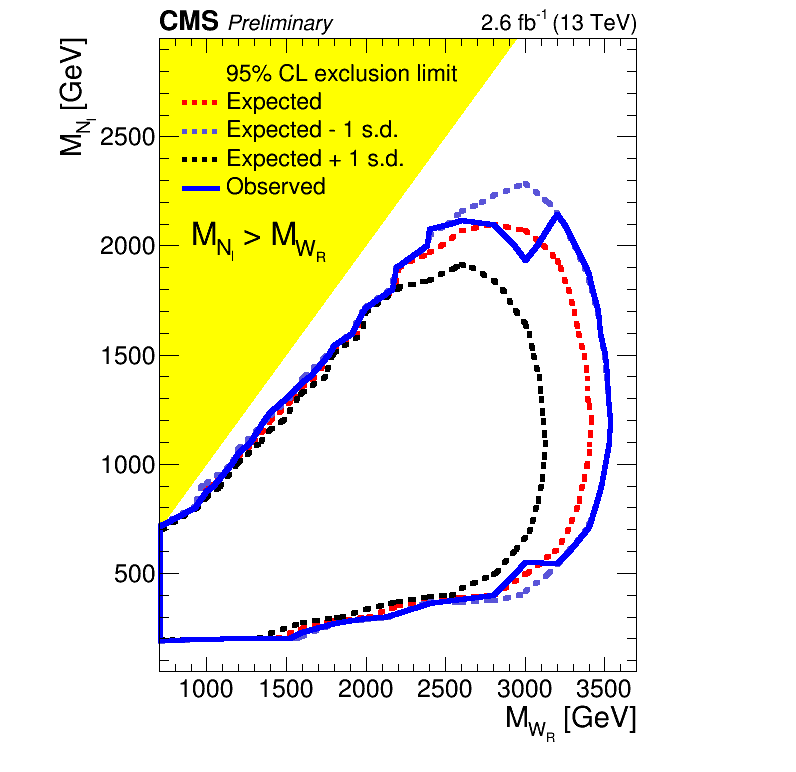
\includegraphics[width=0.65\textwidth]{figures/lim2dWRmumujj_SHv19700toysAprilTwentyThree_exclusionOverlayWithExpPlusMinusOneSigma.png}
  }
  \caption{Exclusion limits on \mWR and \mnul at 95\% CL for $\WR \rightarrow eejj$ (left) and $\WR \rightarrow \mu\mu jj$ (right).}
  \label{fig:twoDimLimits}
 
\end{figure}

The difference between $\chi^'$ and $\chi$ was checked by running full simulations of $\WR \rightarrow \ell\ell jj$, 
including detector response and particle reconstruction, with $\mWR =$ 2400 and 4000 $\GeV$ and several $\mnul \neq \frac{1}{2}\mWR$.  
Simulated events were selected with the full event selection, including trigger and ID requirements, and limits $L_{true}$ on 
$\sigma(\WR) \times BR(\WR \rightarrow \ell\ell jj)$ were calculated at each $(\mWR, \mnul)$ point.  For $\mnul \gtrsim \frac{1}{8}\mWR$, 
$L_{true}$ and $L'$ were consistent within their uncertainties.  For $\mnul \lesssim \frac{1}{8}\mWR$, $L'$ was weaker (the 
minimum excluded \mnul was higher) than $L_{true}$ because of pileup jets.  The simulations used to calculate $L_{true}$ included 
pileup interactions (on average 10 for every simulated event), and pileup jets enabled more \WR events to pass the full 
selection, which extended the excluded \WR production region to lower \mnul values.  The event selection was known to have low 
signal selection efficiency, $\chi \lesssim 10\%$, for all \mWR with $\mnul \lesssim \frac{1}{8}\mWR$, so in this low \mnul 
region no correction was applied to bring the limits $L'$ and $L_{true}$ into better agreement.

Using data collected in 2015 \mWR production is excluded at 95\% CL for $\mWR \lesssim 3500 (3300) \GeV$ in the $\mu\mu$ 
($ee$) channel.  These exclusion limits are consistent with expectations of the ST, and extend the mass limits in the $\mu\mu$ 
($ee$) channel 400 $\GeV$ (400 $\GeV$) higher in \mWR, and 150 $\GeV$ (300 $\GeV$) higher in \mnul relative to the Run I limits.


%%%%%%%%%%%%%%%%%%%%%%%%%%%%%%%%%%%%%%%%%%%%%%%%%%%%%%%%%%%%%%%%%%%%%%%%%%%%%
